\subsection{Recording ImageJ macro functions}
There are many commands in ImageJ. In the native ImageJ distribution, there are ca. 500 commands. In the Fiji distribution, there are 900+ commands. Some plugins are not macro-ready, but almost all of these commands can be accessed by build-in macro functions. That is great, but we then encounter a problem: how do we find a macro function that does what we want to do?

To show you how to find a function, we write a small macro that creates a new image, adds noise, blurs this image by Gaussian blurring, and then thresholds the image. There is a convenient tool called \textbf{Command Recorder}. 
Do \ijmenu{[PlugIns -> Macros -> Record\ldots]}. A window shown in figure
\ref{fig_macroRecorderBlank} opens.

\begin{figure}[htbp]
\begin{center}
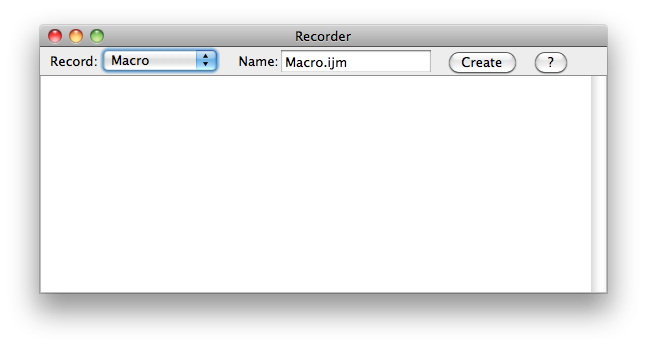
\includegraphics[scale=0.6]{fig/MacroRecorderBlank.png}
\caption{Macro Recorder} \label{fig_macroRecorderBlank}
\end{center}
\end{figure}

All the menu commands that you execute will be printed out as a history of macro functions in this window. For composing a macro using this recorder, we first do the processing manually from the menu as follows. 
\begin{itemize}
  \item Prepare a new image using \ijmenu{[File -> New]} command. The size of the image can be anything.
  \item Then do \ijmenu{[Process -> Noise -> Salt and Pepper]} (Fig.
  \ref{fig_SaltAndPepper}).
  \item \ijmenu{[Process -> Filters -> Gaussian Blur]} (use Sigma = 2.0).
  \item \ijmenu{[Image -> Adjust -> Threshold\ldots]}. Toggle the slider to make
  signals red. Check "Dark Background", then click "Apply".
\end{itemize}
 
\begin{figure}[htbp]
\begin{center}
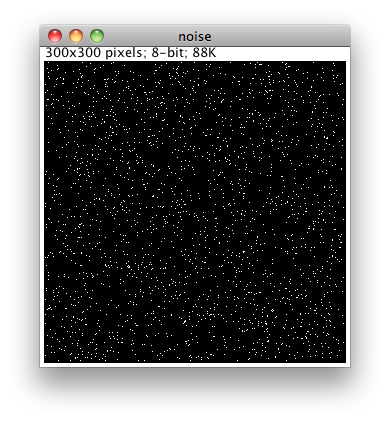
\includegraphics[scale=0.6]{fig/SaltandPepper300.png}
\caption{A demo image for Recording Macro} 
\label{fig_SaltAndPepper}
\end{center}
\end{figure}

Now, check the Command Recorder window. 
It should look like Fig. \ref{fig_macroRecorderFilled}. 
Each line is a macro function that corresponds to a menu command you selected.

\begin{figure}[htbp]
\begin{center}
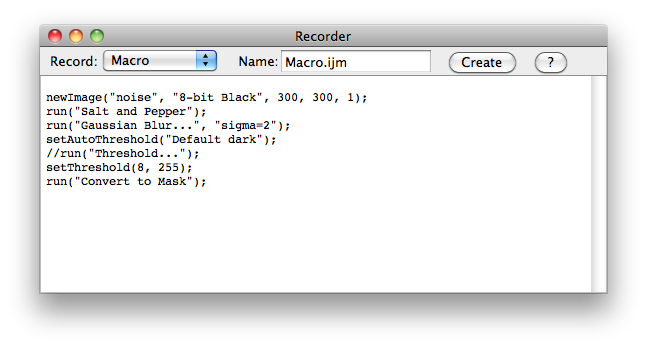
\includegraphics[scale=0.6]{fig/MacroRecorderFilled.png}
\caption{Macro Recorder after some lines Recorded} 
\label{fig_macroRecorderFilled}
\end{center}
\end{figure}

These texts generated in the recorder can be used as it is in your macro.  You could copy and paste them\footnote{In case of OSX, you might probably need to click ``Create'' button to generate a duplicate of macro functions in a new script window. Then you could copy the macro functions from there.}. Compose a macro like below by copying and pasting the macro functions in the recorder.  Delete the lines that are commented out (lines that begin with "//" are lines that are skipped by the macro interpreter).
\lstinputlisting{code/code06_9.ijm}

Run the macro! \ldots I hope that you are amazed by now with the power of Macro
Recorder! Next, you could simply add a line with curly braces at the top and bottom, to package macro commands in a named macro. This is optional in the current case, but it's always a good practice to keep your macro packaged since the boundary of the macro becomes clear. 
 
\lstinputlisting{code/code07.ijm}

The third line in the above macro has a function \ilcom{newImage()}. This
function creates a new image. It has five arguments (in coding jargon, we say
there are "five arguments"). To know what these arguments are, 
the quickest way is to read the Build-In Macro Function page in ImageJ web site\footnote{\url{http://rsbweb.nih.gov/ij/developer/macro/functions.html}}.  
The description of the function \ilcom{newImage} looks like this. 

\begin{indentCom}

\fbox{
\parbox[b][16em][c]{0.80\textwidth}{
\textbf{newImage}(title, type, width, height, depth)\\
Opens a new image or stack using the name title. 
The string type should contain "8-bit", "16-bit", "32-bit" or "RGB". 
In addition, it can contain "white", "black" or "ramp" (the default is "white"). 
As an example, use "16-bit ramp" to create a 16-bit image containing a grayscale ramp.  Width and height specify the width and height of the image in pixels.  Depth specifies the number of stack slices.
}}
\end{indentCom}
Using this information, you can modify the macro to change the size of the image.

\begin{indentexercise}{1}
Modify the code 7 and try changing the size of window to be created.

\item \textbf{Answer}: Change the 3rd line as shown below. It will create a image with 500 pixels width and 200 pixels height image.  
	\begin{lstlisting}[numbers=none]
		newImage("test", "8-bit Black", 500, 200, 1);
	\end{lstlisting}
\end{indentexercise}

Other optional lines you could add to the macro are ``comments''. This does not affect the macro but adding some comment about what the macro does helps you to understand what the macro is doing when you open the file some time later. There are two ways to add comment. One is the \textbf{block comment}. Texts bounded by \ilcom{ /*} and \ilcom{*/} will be ignored by interpreter. Another is the line comment. Texts in a line starting with double slash \ilcom{//} will be ignored by the interpreter. Below is an example of commenting code 07. 

\lstinputlisting{code/code07_1.ijm}
